\section{The Analysis of Security and Privacy}
\label{sec:analysis}
%In this section, we presents the analysis that UPPRESSO achieves the required properties of security and privacy.


\subsection{Security}
UPPRESSO satisfies the security requirements of SSO identity tokens \cite{ArmandoCCCT08,FettKS16, FettKS17},
     explained in Section \ref{subsec:basicrequirements}.
\begin{itemize}
\setlength{\topsep}{0pt}
\setlength{\partopsep}{0pt}
\setlength{\itemsep}{0pt}
\setlength{\parsep}{0pt}
\setlength{\parskip}{0pt}
\item  \textbf{RP Designation}~The RP (pseudo-)identity bound in the identity token
     identifies the target RP, and only this RP.
\item \textbf{User Identification}~The user (pseudo-)identity bound in the identity token identifies
        the authenticated user, and only this user.
\item \textbf{Confidentiality}~An identity token
    is accessible to only
                the authenticated user, the target RP, and the IdP.
\item \textbf{Integrity}~An honest RP accepts only identity tokens binding its (pseudo-)identity and the authenticated user's (pseudo-)identity.
           % and any forged or modified identity token will be rejected.
\end{itemize}


\noindent\textbf{RP Designation.}
The identity token binds $PID_{RP}$ identifying the target RP,
    because $t$ is sent to the target RP with $ID_{RP}$ and $PID_{RP} = [t]ID_{RP}$.


Next, based on the ECDLP
    we prove that,
    for an adversary,
        the probability of finding $t$ and $t'$
    satisfying $[t]ID_{RP_j} = [t']ID_{RP_{j'}}$ is negligible,
    where $RP_j$ and $RP_{j'}$ are any two RPs in the finite set of RPs (i.e.,
    $ID_{RP_j} = [r_j]G$ and $ID_{RP_{j'}} = [r_{j'}]G$, while $r_j$ and $r_{j'}$ are kept secret to adversaries).
This negligible probability means the token designates \emph{only} the target RP.

Let $\mathbb{E}$ be an elliptic curve, %over a finite field $\mathbb{F}_q$,
    $G$ be a point on $\mathbb{E}$ of order $n$,
        and $Q = [x]G$ where $x$ is a random integer in $\mathbb{Z}_n$.
Given $G$ and $Q$,
    the probability that a probabilistic polynomial time (PPT) algorithm calculates $x$ (i.e., solve the ECDLP) is negligible.
For any PPT algorithm $\mathcal{D}$ to calculate $x$, we define
\begin{equation*}
{\rm Pr}\{\mathcal{D}(G, [x]G)=x\} = \epsilon_{c}(k)
\end{equation*}
Here, ${\rm Pr}\{\}$ denotes the probability.
So $\epsilon_{c}(k)$ becomes negligible with the increasing security parameter $k$.

Assume a game $\mathcal{G}_c$ between an adversary and a challenger,
    to describe this $PID_{RP}$ collision attack:
the adversary receives a finite set of RP identities from the challenger,
 denoted as ($ID_{RP_1}$, $ID_{RP_2}$, ..., $ID_{RP_m}$)
 where $m$ is the amount of RPs in the system,
  and then outputs $(a, b, t, t')$.
If $[t]ID_{RP_a}=[t']ID_{RP_b}$, the adversary succeeds in this game.
%If the adversary has the non-negligible probability on succeeding in this game, RP designation is broken.
Note that $m$ is a finite integer, and $m \ll 2^k$ as $k$ increases.
We define the probability that the adversary succeeds in this game as ${\rm Pr}_s$.


\begin{figure}[tb]
  \centering
  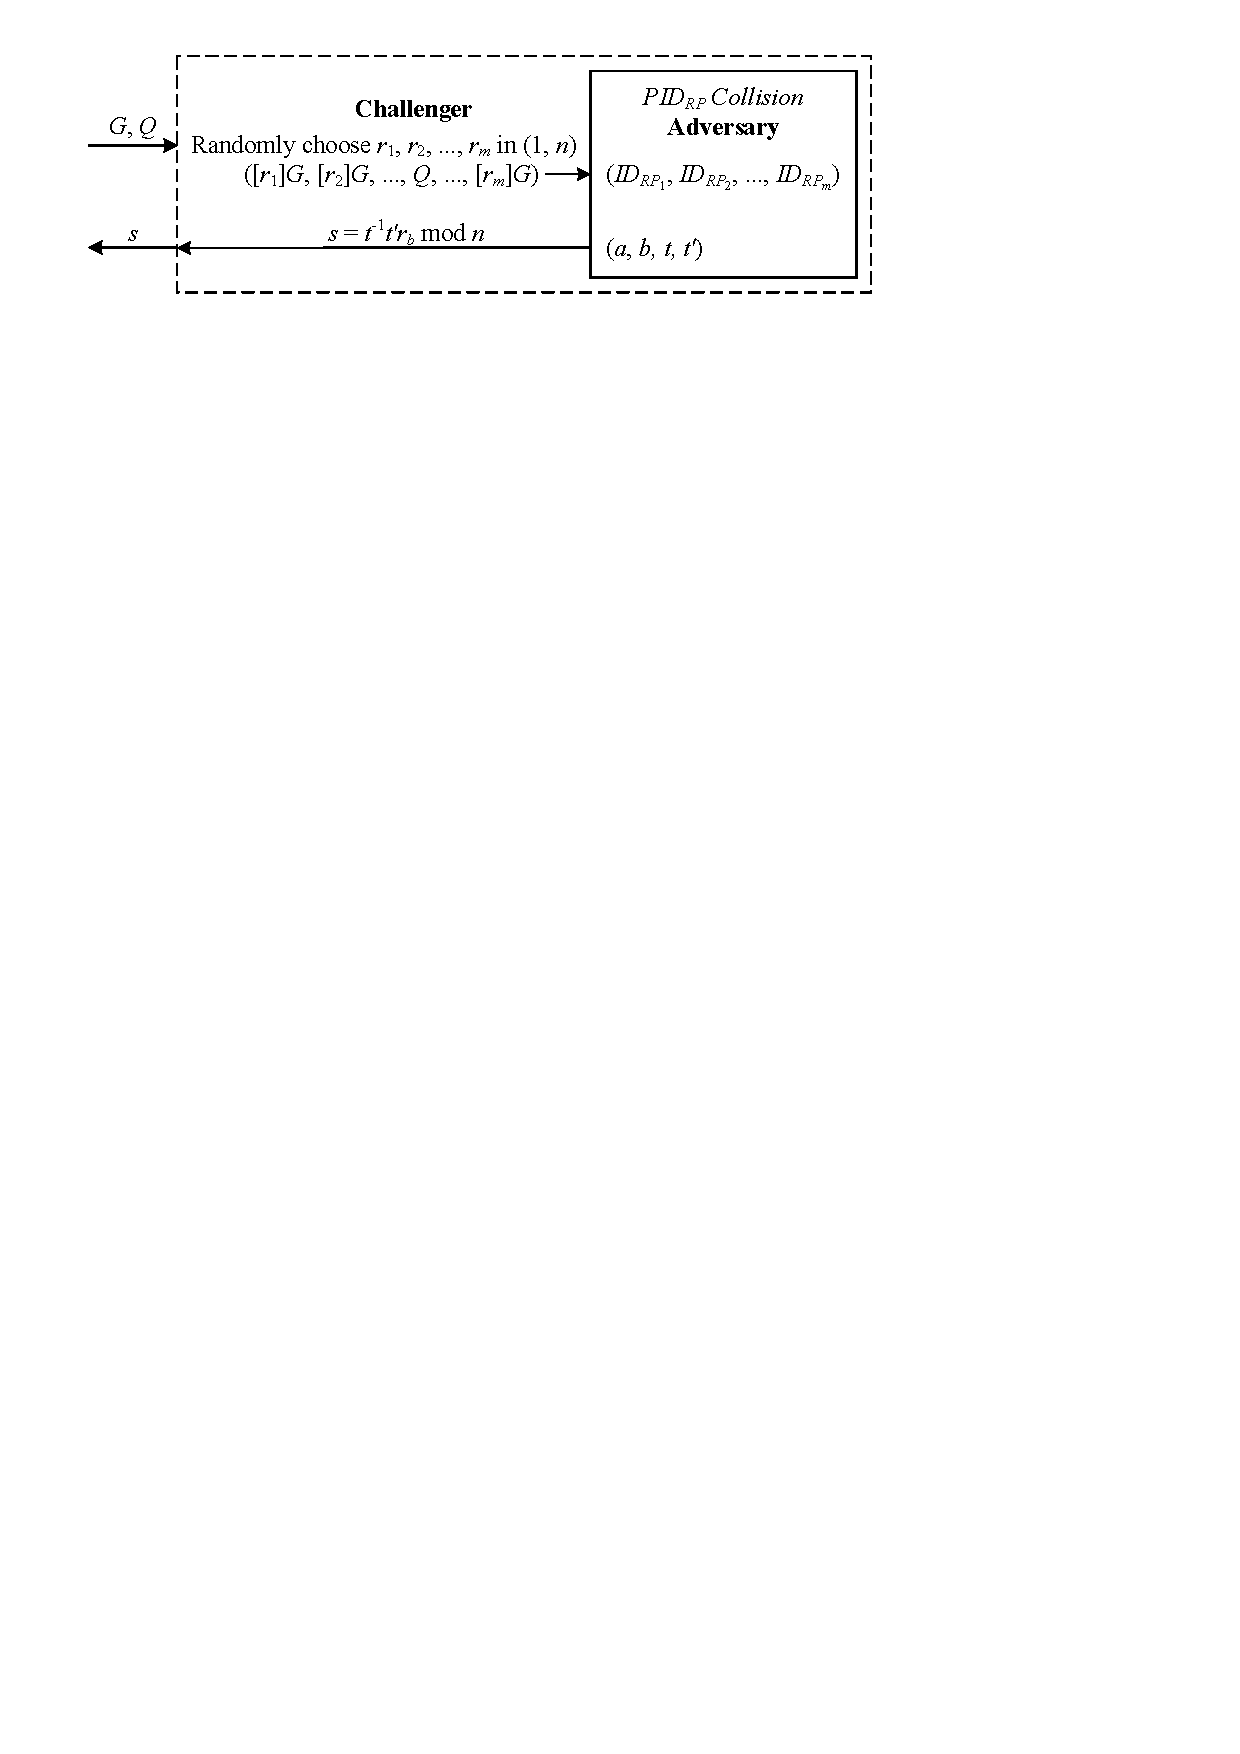
\includegraphics[width=0.96\linewidth]{fig/ecdlp_algorithm.pdf}
  \caption{The algorithm based on the $PID_{RP}$ collision, to solve the ECDLP.}
  \label{fig:ecdlp_algorithm}
\end{figure}


Figure~\ref{fig:ecdlp_algorithm} shows a PPT algorithm $\mathcal{D}^*_c$ based on this game, to solve the ECDLP.
The input of $\mathcal{D}^*_c$ is in the form of ($G$, $Q$).
On receiving an input, the challenger of $\mathcal{G}_c$ randomly chooses $r_1, r_2, \cdots, r_m$ in $\mathbb{Z}_n$,
 calculates $[r_1]G, [r_2]G, \cdots, [r_m]G$,
 and randomly replaces some $[r_j]G$ with $Q$.
Then,
    these $m$ RP identities are sent to the adversary,
which returns the result ($a$, $b$, $t$, $t'$).
Finally, the challenger calculates $s = t^{-1}t'r_b \bmod n$ and returns $s$ as the output of $\mathcal{D}^*_c$.

If $[r_a]G$ happens to be replaced with $Q$ and the adversary succeeds,
    we find $Q = [s]G$ and then $s=x$ because $[tr_a]G = [t]Q = [t'r_b]G$.
As $[r_j]G$ is randomly replaced by the challenger,
    $Q$ and other RP identities in the input set are indistinguishable to the adversary.
Thus,
\begin{align*}
&{\rm Pr}\{\mathcal{D}^*_c(G, [x]G)=x\} = {\rm Pr}\{s = x\}\\=&{\rm Pr}\{a=j\}{\rm Pr}_s=\frac{1}{m}{\rm Pr}_s
\end{align*}

If the adversary is able to find $t$ and $t'$
    satisfying that $[t]ID_{RP_j} = [t']ID_{RP_{j'}}$,
    it will have non-negligible advantages in $\mathcal{G}_c$
        and then
         ${\rm Pr}_s$ becomes non-negligible as $k$ increases.
Because $m \ll 2^k$, ${\rm Pr}\{\mathcal{D}^*_c(G, [x]G)=x\} = \frac{1}{m}{\rm Pr}_s$ also
becomes non-negligible with the increasing $k$.
This violates the ECDLP assumption.
Thus, the probability of finding $t$ and $t'$ satisfying that $[t]ID_{RP_j} = [t']ID_{RP_{j'}}$ in UPPRESSO is negligible,
    and then adversaries cannot break RP designation.


%If ${\rm Pr}_s$ is non-negligible with the security parameter $k$, ${\rm Pr}\{\mathcal{D}^*_c(G, [x]G)=x\} =\frac{1}{m}{\rm Pr}_s$ is also non-negligible because $m << 2^k$,
%which means that $\mathcal{D}^*_c$ solves the ECDLP.
%So the adversary does not have non-negligible advantages in $\mathcal{G}_c$,
%    and the probability of finding $t$ and $t'$
%    satisfying that $[t]ID_{RP_j} = [t']ID_{RP_{j'}}$ in UPPRESSO is negligible.


%An identity token binding $PID_U$ and $PID_{RP}$,
%    designates the target RP, and only the target RP.
%An honest RP calculates $PID_{RP}$ by itself with the trapdoor $t$ sent from the user,
%    and checks $PID_{RP}$ in the $PID_{RP}$-registration result and the identity token.
%So the target RP will accept this token.

%Meanwhile,
%        the honest IdP guarantees that, within its validity period, the $PID_{RP}$ will be registered only once.
% $PID_{RP}$ will be bound in some identity token.
%An honest RP is ready to accept an identity token binding $PID_{RP}$, only after it receives the signed $PID_{RP}$-registration result.
%Because (\emph{a}) both $PID_{RP}$ and $H(t)$ in the registration result are checked by the RP and then (\emph{b}) the registration result $[PID_{RP}, H(t), Validity]_{SK}$ is acceptable to only one honest RP,
%            the identity token designates only one RP.

\vspace{0.8mm}
\noindent\textbf{User Identification.}
Given a user, an honest RP with $ID_{RP}$ always deterministically derives an identical account from different identity tokens binding $PID_U$ and $PID_{RP}$.
That is,
    in the user's any $i$-th and $i'$-th ($i \neq i'$) login instances to the RP,
 $\mathcal{F}_{Acct}(PID_{U}^i, PID_{RP}^i) = \mathcal{F}_{Acct}(PID_{U}^{i'}, PID_{RP}^{i'}) = [ID_U]ID_{RP}$.

In the calculation of $Acct = [t^{-1}]PID_U = [t^{-1}][u]PID_{RP}$,
%$t$ and $PID_{RP}$ have been checked by the honest RP in the $PID_{RP}$-registration result,
$PID_U$ is calculated by the honest IdP based on (\emph{a}) the authenticated user, i.e., $ID_U = u$, and (\emph{b}) the received $PID_{RP}$, while this $PID_{RP}$ is generated by the target RP based on $ID_{RP}$ and $t$.
Thus, the calculated account is always exactly the authenticated user's account at the RP (i.e., $[ID_U]ID_{RP}$).
%Moreover, adversary may try to provide the
%However, according to the proof of RP designation, there would not be the generated $t$ and $t'$ happening to satisfy that $PID_{RP} = [t]ID_{RP_j} = [tr]G = [t'r']G = [t']ID_{RP_{j'}}$.


%Two malicious users, whose identities are $ID_U = u$ and $ID_{U'} = u'$,
%    could attempt to login to $RP_j$ and $RP_{j'}$, respectively.
%If the generated $t$ and $t'$ happen to satisfy that $PID_{RP} = [t]ID_{RP_j} = [tr]G = [t'r']G = [t']ID_{RP_{j'}}$,
%    these collusive users could arbitrarily choose to register either $[PID_{RP}, PEnpt_U, H(t)]$ or $[PID_{RP}, PEnpt_{U'}, H(t')]$ at the IdP,
%        to receive an identity token binding $PID_{RP}$ and either $PID_U = [u]PID_{RP}$ or $PID_{U'} = [u']PID_{RP}$.\footnote{Such a token designates either $RP_j$ or $RP_{j'}$,
%    but only one honest RP because there is only one acceptable $PID_{RP}$-registration result which is signed by the IdP.
%    So RP designation is not violated in this attack case.}
%When such a token is signed for $RP_j$, the calculated $Acct$ is $[ur]G$ or $[u'r't't^{-1}]G = [u'r]G$;
%    or, when it is signed for $RP_{j'}$, $[urtt'^{-1}]G = [ur']G$ or $[u'r']G$ is calculated.
%That is,
%        even in this collusive case,
%    the calculated account is still the authenticated user's account at the target RP,
%    and it does not result in any attack.


%An adversary might try allure a user to login under the adversary's account,
%    by injecting his identity token into the user's communications with an honest RP.
%Such identity injection attacks are impossible in UPPRESSO as follows.
%If the negotiation of $PID_{RP}$ is not finished yet,
%    the RP will reject the malicious token.
%Even when $PID_{RP}$ has been negotiated,
%    it is kept unknown to the adversary because the communications between two scripts are controlled by a browser
%     and the communications between the browser and the IdP (or the RP) are protected by TLS.
%Thus, an adversary cannot obtain $PID_{RP}$ dynamically negotiated between an honest RP and the user,
%     so it cannot construct an identity token acceptable to the RP.
%

\vspace{0.8mm}
\noindent\textbf{Confidentiality.}
No event leaks an identity token to any malicious entity other than the authenticated user and the designated RP.
First of all, the communications among the IdP, RPs and users,
    are protected by HTTPS,
    and the \verb+postMessage+ HTML5 API ensures the dedicated channels between two scripts within the browser,
    so adversaries cannot eavesdrop the identity tokens.
Further, the IdP sends the identity token only to the authenticated user
        (i.e., the IdP script).
The IdP script forwards the token to the RP script
 only if it is downloaded from the same origin as $Enpt_{RP}$,
and the binding of $Enpt_{RP}$ and $ID_{RP}$ is ensured by the signed RP certificate.
  %  which is verified by the IdP script.
So only the RP that holds $Enpt_{RP}$ and $ID_{RP}$,
    receives this token.


%The detailed process of proof is shown in Appendix.
\vspace{0.8mm}
\noindent\textbf{Integrity.}
The identity token binds $Acct$ and $ID_{RP}$ implicitly,
    and any breaking results in some failed check or verification in the login flow.
%It is ensured by the IdP's signatures:
The identity token binding $PID_U$ and $PID_{RP}$ is signed by the IdP.
According to the proof of RP designation,
    there is no $t' \neq t$ but satisfying that $PID_{RP} = [t]ID_{RP_j} = [t']ID_{RP_{j'}}$.
That is, the identity token explicitly binding $PID_U$ and $PID_{RP}$,
    matches \emph{only} one $ID_{RP}$ and then also \emph{only} one $Acct = [t^{-1}]PID_{U}$.
Thus,
    $Acct$ and $ID_{RP}$ are actually bound by the IdP's signatures,
        due to the one-to-one mapping between (\emph{a}) the pair of $Acct$ and $ID_{RP}$ and (\emph{b}) the triad of $PID_U$, $PID_{RP}$, and $t$.

%The detailed process of proof is shown in Appendix.

%The detailed process of proof is shown in Appendix.

\vspace{1mm}
Finally, we have formally analyzed the security properties of UPPRESSO, %especially confidentiality and integrity,
     based on a Dolev-Yao style model \cite{SPRESSO}.
% which has been used in the formal analysis of SSO protocols such as OAuth 2.0 \cite{FettKS16} and OIDC \cite{FettKS17}.
The model abstracts the entities in a web system,
    such as web servers and browsers,
    as \emph{atomic processes}. %which communicate with each other through events. % such as HTTPS request and response.
It defines \emph{script processes} to formulate client-side scripts.
%The script is dependently invoked by the browser to process the server-defined logic.
  %such as verifying $Certificate_{RP}$.

%postmessage events;

%atomic process <-> script process, communication.

%Other events change self-trigger.

The UPPRESSO system contains atomic processes as follows:
an IdP process,
    a finite set of web servers for honest RPs, a finite set of honest browsers, and a finite set of attacker processes.
These processes communicate with each other through events such as HTTPS request and response.
We consider all RP and browser processes are honest,
 while model an RP or a browser controlled by an adversary as attacker processes.
Within a browser,
 honest IdP scripts, honest RP scripts and also attacker scripts are invoked.
%Although the scripts coexist in the same browser, they are strictly separated.
Script processes communicate with each other through \verb+postMessage+,
    modelled as transmitted-to-itself events of the browser process.
%To clearly indicate the action of postMessage communication, we define it as the transmitting-to-itself event of the browser (which is not defined in SPRESSO).

%It contains two honest script processes,
%        downloaded from the RP process and the IdP process, respectively.
% and {\sf script\_attacker} denotes a script downloaded by an attacker process that exists in all browser processes.
%attacker script processes

After formulating UPPRESSO by the Dolev-Yao style model,
    we trace the whole lifecycle of an identity token,
        starting when it is generated and ending when accepted by the RP,
 to ensure the token is not leaked to attackers or tampered with by any adversary.
We locate the generation of an identity token, and trace to all places
    where $PID_U$, $PID_{RP}$ and other parameters in the token are calculated and transmitted,
     to ensure no adversary retrieves or manipulates them.
%The tracing also confirms no adversary retrieves the token.

%The details on the Dolev-Yao web model and the detailed security proofs of UPPRESSO are in the appendix.

%Finally,
%    we formally prove that,
%\emph{user identification}, \emph{RP designation}, \emph{confidentiality}, and \emph{integrity} are fulfilled in UPPRESSO.


\subsection{Privacy}
UPPRESSO effectively prevents the threats of IdP-based login tracing and RP-based identity linkage.

\vspace{0.8mm}
\noindent\textbf{IdP-based Login Tracing.}
The information accessible to the IdP and derived from the RP's identity,
    is only $PID_{RP}$, where $PID_{RP} = [t]ID_{RP}$ is calculated by the user.
Because  (\emph{a}) $t$ is a random number from $\mathbb{Z}_n$ and kept secret to the IdP
 and (\emph{b}) $ID_{RP} = [r]G$ and $G$ is the base point (or generator) of $\mathbb{E}$,
 the IdP has to view $PID_{RP}$ as randomly and independently chosen from $\mathbb{E}$,
    and cannot distinguish $[t]ID_{RP_j} = [tr]G$ from any $[t']ID_{RP_{j'}} = [t'r']G$.
So, the IdP cannot infer the RP's identity or link any pair of $PID_{RP}^i$ and $PID_{RP}^{i'}$,
    and the IdP-based login tracing is impossible.

\vspace{0.8mm}
\noindent\textbf{RP-based Identity Linkage.}
We prove UPPRESSO prevents the RP-based identity linkage,
 based on the elliptic curve decision Diffie-Hellman (ECDDH) assumption. %\cite{GoldwasserK16}.
%That is, while there is the login to an RP, for colluded RPs, they cannot decide whether this login and any logins to other RPs are from the same user.
%
Let $\mathbb{E}$ be an elliptic curve,
    and $G$ be a point on $\mathbb{E}$ of order $n$.
For any PPT algorithm $\mathcal{D}$, the probability of distinguishing
 $([x]G$, $[y]G$, $[xy]G)$ and $([x]G$, $[y]G$, $[z]G)$
is negligible,
 where $x$, $y$ and $z$ are integers randomly and independently chosen from $\mathbb{Z}_n$.
Let  ${\rm Pr}\{\}$ denote the probability and
 we define
\begin{align*}
&{\rm Pr}_1 =  {\rm Pr}\{\mathcal{D}(G, [x]G, [y]G, [xy]G)=1\} \\
&{\rm Pr}_2 =  {\rm Pr}\{\mathcal{D}(G, [x]G, [y]G, [z]G)=1\}
\end{align*}
So $\epsilon_{r}(k) = |{\rm Pr}_1 - {\rm Pr}_2|$ becomes negligible as $k$ increases.


In every login instance,
    the RP holds $ID_{RP}$ and $Acct$, receives $t$, calculates $PID_{RP}$,
    and verifies $PID_{RP}$ and $PID_U$ in the identity token.
After filtering out the redundant information (i.e., $PID_{RP}= [t]{ID_{RP}}$ and $Acct = [t^{-1}]PID_{U}$),
    the RP actually receives $(ID_{RP}, t, Acct) = ([r]G, t, [ur]G)$.

The prevention against the RP-based identity linkage is proved
    by this proposition:
when $c$ collusive RPs collect the information of login instances by $v$ users,
    they still cannot determine whether a login instance to another RP belongs to one of these $v$ users or not.
The collected login instances are expressed as $\mathfrak{L}=\left\{ \begin{matrix}
L_{1,1}, & L_{1,2}, & \cdots, & L_{1,c}\\
L_{2,1}, & L_{2,2}, & \cdots, & L_{2,c}\\
\cdots, & \cdots, & \cdots, & \cdots\\
L_{v,1}, & L_{v,2}, & \cdots, & L_{v,c}
\end{matrix}\right\}$, where $L_{i, j} = (ID_{RP_j}, t_{i, j}, [ID_{U_i}]{ID_{RP_j}}) = ([r_j]G, t_{i,j}, [u_ir_j]G)$.
Given a login instance to another RP $L'=(ID_{RP_{c+1}}, t', [ID_{U'}]ID_{RP_{c+1}}) = ([r_{c+1}]G, t', [u'r_{c+1}]G)$,
we define the RP-based identity linkage game $\mathcal{G}_r$:
after receiving $\mathfrak{L}$ and $L'$ from a challenger,
    the adversary outputs the result $s = 1$ if it determines that $u' \in \{u_1, u_2, \cdots, u_v\}$,
        or $s = 0$ otherwise.


We define the adversary's advantage in $\mathcal{G}_r$ as $\mathbf{Adv}_A$.
%If the adversary is able to distinguish whether $u' \in \{u_1, u_2, \cdots, u_v\}$ or not,
%    the adversary will have non-negligible advantages in $\mathcal{G}_r$
%        and ${\rm Adv}_A$ is non-negligible.
Then,
\begin{align*}
&{\rm Pr}'_1={\rm Pr}\{\mathcal{G}_r(\mathfrak{L}, L'|ID_{U'} \in \{ID_{U_1}, ID_{U_2}, \cdots, ID_{U_v}\})=1\} \\
&{\rm Pr}'_2={\rm Pr}\{\mathcal{G}_r(\mathfrak{L}, L'|ID_{U'} \in \mathbb{Z}_n)=1\}\\
&{\mathbf{Adv}}_A=|{\rm Pr}'_1-{\rm Pr}'_2|
\end{align*}

We design a PPT algorithm $\mathcal{D}^*_r$ based on $\mathcal{G}_r$, shown in Figure~\ref{fig:dalgorithm}, to solve the ECDDH problem.
The input is in the form of $(G$, $Q_1=[x]G$, $Q_2=[y]G$, $Q_3=[z]G)$.
On receiving the input, the challenger of $\mathcal{G}_r$ randomly chooses
 $\{u_1, u_2, \cdots, u_v\}$, $\{r_1, r_2, \cdots, r_c\}$, $\{t_{1, 1}, t_{1, 2}, \cdots, t_{v, c}\}$, and $t'$ from $\mathbb{Z}_n$.
Then the challenger constructs $\mathfrak{L}$ and $L'$ as below.
It first assigns $L_{i, j} = ([r_j]G, t_{i, j}, [u_ir_j]G)$, %$1\leq i \leq v$ and $1\leq j \leq c$,
    and randomly chooses $d \in [1, v]$ to
 replace $[u_d r_j]G$ with $[r_j]Q_1=[xr_j]G$ for $1\leq j \leq c$.
So $\mathfrak{L}=\left \{ \begin{matrix}
L_{1,1},&L_{1,2},&\cdots,&L_{1,c}\\
L_{2,1},& L_{2,2},&\cdots,&L_{2,c}\\
\cdots,&\cdots,&\cdots,&\cdots\\
([r_{1}]G, t_{d, 1}, [r_{1}]Q_1),&\cdots,&\cdots,&([r_{c}]G, t_{d, c}, [r_{c}]Q_1)\\
\cdots,&\cdots,&\cdots,&\cdots\\
L_{v,1},&L_{v,2},&\cdots,&L_{v,c}
\end{matrix}\right\}$.
%$L=$\{($[r_1]G$, $t_{1, 1}$, $[[u_1][r_1]G$), ($[r_2]G$, $t_{1, 2}$, $[u_1][r_2]G$), $\cdots$, ($[r_{\beta}]G$, $t_{\alpha, \beta}$, $[r_{\beta}]Q_1$), $\cdots$, ($[r_b]G$, $t_{a, b}$, $[u_a][r_b]G$)\}
%
Next, it constructs $L' = (Q_2, t', Q_3) = ([y]G, t', [z/y][y]G)$.
Finally,
    $\mathfrak{L}$ and $L'$ are sent to the adversary,
        and the output $s$ of $\mathcal{G}_r$ is output by the challenger.
According to the above construction of $\mathfrak{L}$ and $L'$,
    $x$ is actually inserted into $\mathfrak{L}$ as $u_d$
    and $z/y$ is assigned to $u'$.
So, if $z = xy$, then $z/y=x$ and $ID_{U'} \in \{ID_{U_1}, ID_{U_2}, \cdots, ID_{U_v}\}$;
    otherwise, $ID_{U'} \in \mathbb{Z}_n$.
Thus,
\begin{align*}
&{\rm Pr}_1={\rm Pr}\{\mathcal{D}^*_r(G, [x]G, [y]G, [xy]G)=1\}={\rm Pr}'_1 \\=&  {\rm Pr}\{\mathcal{G}_r(\mathfrak{L}, L'|ID_{U'} \in \{ID_{U_1}, ID_{U_2}, \cdots, ID_{U_v}\})=1\} \\
&{\rm Pr}_2={\rm Pr}\{\mathcal{D}^*_r(G, [x]G, [y]G, [z]G)=1\} ={\rm Pr}'_2 \\=&  {\rm Pr}\{\mathcal{G}_r(\mathfrak{L}, L'|ID_{U'} \in \mathbb{Z}_n)=1\}\\
&{\mathbf{Adv}}_A=|{\rm Pr}'_1-{\rm Pr}'_2|=|{\rm Pr}_1-{\rm Pr}_2|=\epsilon_{r}(k)
\end{align*}

\begin{figure}[tb]
  \centering
  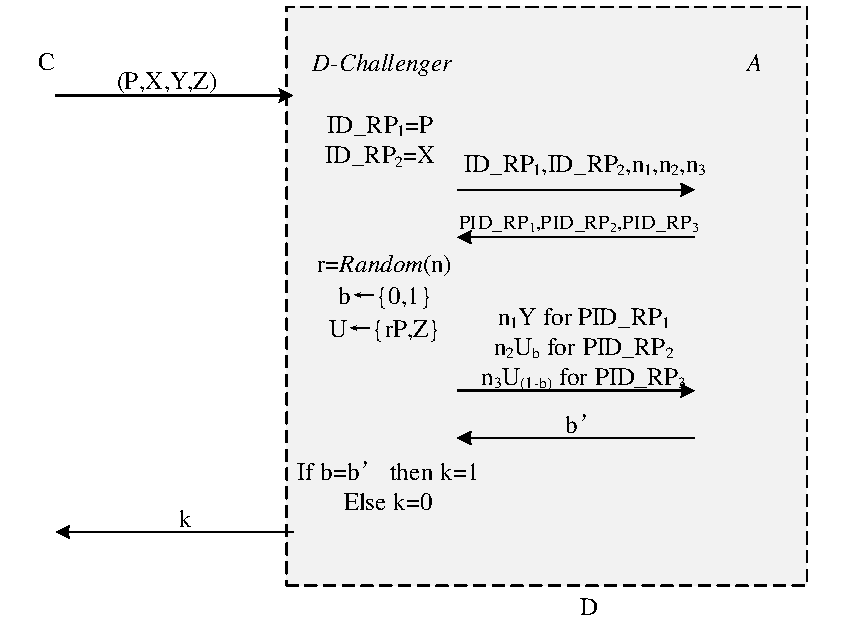
\includegraphics[width=0.96\linewidth]{fig/dalgorithm.pdf}
  \caption{The algorithm based on the RP-based identity linkage, to solve the ECDDH problem.}
  \label{fig:dalgorithm}
\end{figure}

The ECDDH assumption means that in $\mathcal{G}_r$ the adversary does not have advantages,
    i.e., cannot distinguish a user $U'$ chosen from \{${U_1}, {U_2}, \cdots, {U_v}$\}
        or randomly from the user set of UPPRESSO.
%    (indistinguishability of users to collusive RPs).
So the RP-based identity linkage is impossible.

%    the adversary will have non-negligible advantages in $\mathcal{G}$
%        and $Pr_s$ is non-negligible.

%If $s'=1$ and $ID_U' \in$\{$ID_{U_1}$, $ID_{U_2}$, ..., $ID_{U_a}$\}, the adversary succeeds in this game.
%If the adversary does not have the non-negligible probability on succeeding in this game, RP-based identity linkage is not impossible.

%We define the probability that the adversary succeeds in this game as $Pr_s'$.
%So, if the adversary is able to ,
%    the adversary will have non-negligible advantages in $\mathcal{G}$
%        and $Pr_s$ is non-negligible.
